\documentclass[12pt,oneside]{article}
\usepackage[utf8]{inputenc}
\usepackage{float}
\usepackage[bottom]{footmisc}
\usepackage{bookmark}
\usepackage{microtype}
\usepackage{amsmath}
\usepackage{multicol}
\usepackage{mdframed}
\usepackage{setspace}
\usepackage{pgfplots}
\usepackage{graphicx}
\usepackage{fancyvrb}
\usepackage[absolute]{textpos}\TPGrid{16}{16}
\usepackage{tikz}
  \usetikzlibrary{shapes}
  \usetikzlibrary{arrows.meta}
  \usetikzlibrary{arrows}
  \usetikzlibrary{shadows}
  \usetikzlibrary{trees}
  \usetikzlibrary{fit}
  \usetikzlibrary{calc}
  \usetikzlibrary{positioning}
  \usetikzlibrary{decorations.pathmorphing}
\usepackage{./tikz-uml}
\usepackage{everypage}
  \AddEverypageHook{
    \begin{textblock}{0.5}[0,0](0,0)
      \tikz \node[fill=myred,minimum width=0.5\TPHorizModule,minimum height=16\TPVertModule] {};
    \end{textblock}
    \begin{textblock}{0.125}[0,0](0.5,0)
      \tikz \node[fill=myblack,inner sep=0, minimum width=0.125\TPHorizModule,minimum height=16\TPVertModule] {};
    \end{textblock}
  }
\usepackage{xcolor}
  \definecolor{firebrick}{HTML}{B22222}
  \definecolor{myred}{HTML}{CF0A2C}
  \definecolor{myblack}{HTML}{232527}
\newcommand\dd[1]{\colorbox{gray!30}{\texttt{#1}}}
\usepackage{hyperref}
  \hypersetup{colorlinks=true,allcolors=blue!40!black}
\setlength{\topskip}{6pt}
\setlength{\parindent}{0pt} % indent first line
\setlength{\parskip}{6pt} % before par
% \let\oldsection\section\renewcommand\section{\newpage\oldsection}
\date{\small\today}
\title{%
  DRAFT: DeGit - distributed git repository manager\\
  \colorbox{firebrick}{\small\sffamily\color{white}{White Paper}}}
\usepackage[style=authoryear,sorting=nyt,backend=biber,
  hyperref=true,abbreviate=true,
  maxcitenames=1,maxbibnames=1]{biblatex}
  \renewbibmacro{in:}{}
  \addbibresource{books.bib}
\tikzset{node distance=1.6cm, auto, every text node part/.style={align=center, font={\sffamily\small}}}
\tikzstyle{block} = [draw=myblack, fill=white, inner sep=0.3cm, outer sep=0.1cm, thick]
\tikzstyle{ln} = [draw, ->, very thick, arrows={-triangle 90}, every text node part/.append style={font={\sffamily\scriptsize}}]

% custom commands
\newcommand{\code}[1]{\texttt{#1}}
\newcommand{\todo}[1]{\textcolor{red}{TODO: #1}}

\author{Kirill Chernyavskiy}

\begin{document}
\raggedbottom

\maketitle
\begin{abstract}
Big software companies may have millions of code repositories,
and use them extensively by programmers and CI pipelines.
One git server is not able to satisfy performance expectations,
many servers with load-balancing can't solve this issue too because
of inability storage IO scaling for read operations.
Also, a big company may have distributed teams around the world,
where each team collaborates with others in one git repo,
cross-region repo access could be slow in such cases.
The solution for this problem is distributed git repository storage,
which replicates repositories across region nodes.
\end{abstract}

% \onehalfspace

\section{The problem}

There was an attempt to implement POC distributed repository manager with
eventually consistency guarantee, but it fails because of two reasons:
1) fetch traffic correlates with push frequency because of huge amount of
CI systems involved in development process: each push event usually triggers
CI build which clones the repository.
2) push and fetch frequency is not distributed uniformly over the time: in each
repository, team members may have different responsibilities for review and merge process,
project technical lead can merge all approved pull-requests in short period of time
which causes frequent push operations in git repo.

These two conditions lead to high fetch traffic peaks for git repositories:
frequent push operations turn replication nodes into inconsistent state,
and lead to high fetch traffic from different regions to primary repository node
which can shutdown the node and become the whole repository unavailable for some time.

Merge is not the only way to "update" the repository. Lots of activities can do that,
here is the list of some:

\begin{description}
  \item Create or delete branches by git push or by using web page.
  \item Create or delete tags by git push or by releasing new version on web page.
  \item Developer can update feature branches byself, it can also triggers CI builds.
  \item Tag could be updated using git push.
  \item Special REF create/update: on GitLab, when new merge request is created,
    the new \code{refs/merge-requests/IID/head} named ref
    is created. When source branch of merge request is updated, the ref is also updated.
  \item Migrations: sometimes repository administrator can migrate source code to
    another physical device, it also could be treated as an update.
\end{description}

\section{Solution}

The solution could be the implementation of distributed Git repository manager with
strong consistent replica nodes. It guarantees high availability across
different regions, durability by replicating repositories on different server racks,
read scalability by routing fetch traffic on different nodes.

DeGit is a peer-to-peer system, no persistent master nodes
exists\footnote{The system may have temporary master node for repository elected to perform git command}.
Each node knows about each other due to discovery protocol (\todo{choose discovery protocol}).

Each DeGit node stores multiple repositories on local storage
and exposes RPC API for all git operations. Node can accept RPC operation for repository
which is not located on local storage, in that case it performs lookup
for repository on other nodes and synchronizes it on local storage, and performs RPC command
after that.

When a new repository is created in a system via push operation, the node replicates this repository
to at least 3 other nodes synchronously and propagetes metadata for future repository lookup.

Update operation can be routed to any node which contains the repository. The node synchronously
updates all replicas on push. If update failed due to concurency issue, the whole update fails.

Each node collects usage statistics about fetch and push operation, and system may decide to move repositories
to most frequently used nodes based on this statistics.

The system autmatically rebalances repository storage: when repository is not used actively for a
long time, the node can remove a repository from storage if 3 replicas of this repository exists on other nodes;
if some node has a lot of free space on storage, and storage of another node is almost full,
full node can transfer (move) some repositories to another node.

The system can accept new nodes and automatically fill it with replica repository and
move some repository to new node. Same for dosconnecting: if node was disconnected from the system or crashed,
it creates additional replicas on nodes to have at least 3 replicas for each repository in a system.


\subsection{Protocol}
Main system protocol components are (under discussion):
\begin{description}
  \item[Locators] - unique node identity.
  \item[Network] - node peers connection.
  \item[Discovery] - lookup of node real address by locator ID.
  \item[Metadata] - a mapping of repository to node: a node contains many repositories and
    repository can be replicated across many nodes.
  \item[Git data] - Git objects and references exchange protocol, commands to add new objects and update references.
\end{description}

\subsubsection{Locators}
Each node has peristant public and private keys to identify itself in a system.
Unique identifier\footnote{In this document, node identifier, node-id and node locator refer to the same definition}
is a cryptographic hash of public key of the node in \href{https://multiformats.io/multihash/}{Multihash} format.
Private and public keys can be used to sign requests to other nodes or to build trusted \hyperref[sec:discovery]{discovery}
point in a system: when a new system is created, administrator can create CA (certification authority) for issuing
digital certificates for node public keys, so each node will be able to verify certificate of any other node when
using seed list URLs. Node instances uses locators to talk with each other, it can find real network address of nodes using
this identity. Also, system uses locators for node-repository mapping, the item of mapping table consists of
locator and unique repository name.

Related: "A Practicable Approach Towards Secure Key-Based Routing" by I. Baumgart and S. Mies;
Identities and Network design of IPFS by J. Benet.

\subsubsection{Network}
DeGitX can use different network protocols for RPC calls, \code{TCP} is supported by default
\todo{other protocols, e.g. NAT traversing?}.

\subsubsection{Discovery}
\label{sec:discovery}
Each node doesn't know network addresses of others by default. Different discovery techicues could be used
for node lookup:
\todo{choose the best option}.
\begin{description}
\item[DHT] - distributed hash tables uses different metrics to compare the distance of nodes in overlay network.
  For example \href{pdos.csail.mit.edu/~petar/papers/maymounkov-kademlia-lncs.pdf}{Kademlia} uses
  \code{XOR} metric of node ID for distance measurement. It requires node IDs to be widely distributed -
  DeGitX locators satisfies this requirements, being generated as cryptographic hash function from
  public key. In Kademlia lookup system each node stores references in K-buckets, where each K-bucket
  contains node addresses with same ID prefix. For more details, see section 2.4 of its white paper.
\item[Distributed DB] - network addresses could be propagated to the system using supplimentary distributed
  CP database, e.g. etcd or others. Node registers itself in database on startap, and uses this database for lookups.
  It requires additional system configuration, but delegating some responsibilities to third-party services.
\item[Track host] - nodes can use some central track host to register itself on start. Many track implementations
  provides DNS services to help with discovery of registered nodes.
\item[Hybrid] - system may use different approaches combinations, e.g. discovery service may use distributed database
  and provide single entry point for discovery as track DNS.
\end{description}

\subsection{Metadata}
Repository mapping could be stored in distributed hash table (e.g. Kademlia),
\todo{research and compare different solutions}.

\subsection{Git data exchange}
Consensus could be implemented using \href{https://raft.github.io/raft.pdf}{Raft} or
\href{http://www.cs.yale.edu/homes/aspnes/pinewiki/Paxos.html}{Paxos} algorithm.
\todo{search for more algorithms}.

\subsection{Git Internals}
\subsubsection{Dictionary}
\label{subsec:git-internals}
\begin{description}
  \item[Git] is a simple key-value data store and stores 3 main types of Objects: blob, tree, commit, and one additional: tag.
  \item[Blob] - content of file w/o filename.
  \item[Tree] - A single tree object contains one or more entries, each of which is the SHA-1 hash of a blob or subtree with its associated mode, type, and filename.
  For example, the most recent tree in a project may look something like this:\\
  \\
  \code{\$ git cat-file -p master\^\{tree\}}\\
  \code{100644 blob a906cb2a4a904a152e80877d4088654daad0c859      README}\\
  \code{100644 blob 8f94139338f9404f26296befa88755fc2598c289      Rakefile}\\
  \code{040000 tree 99f1a6d12cb4b6f19c8655fca46c3ecf317074e0      lib}
  \begin{figure}[H]
    \centering
    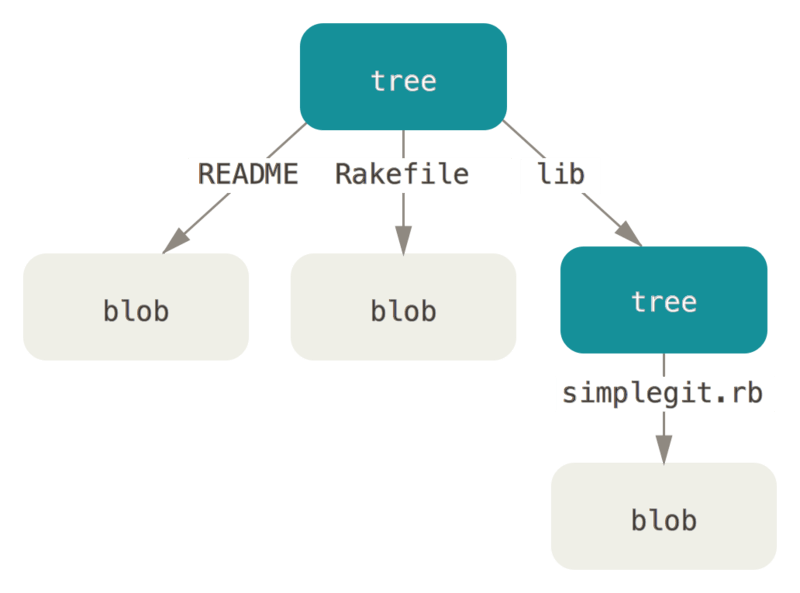
\includegraphics[width=\textwidth]{data-model-1.png}
    \label{fig:tree-objects}
  \end{figure}
  \item [Commit] is just a pointer to parent(previous) commit if any
  and to top-level tree for current one with some metadata
  (the author information and so on).
  \begin{figure}[H]
    \centering
    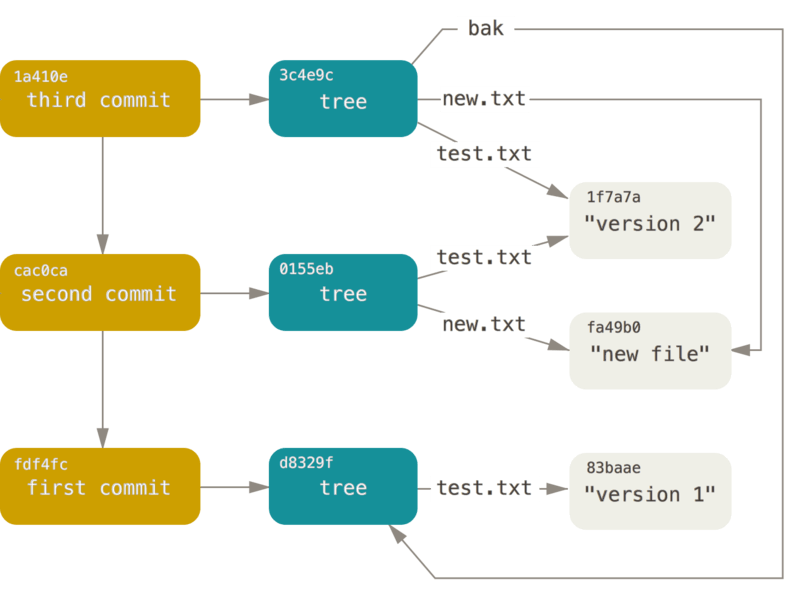
\includegraphics[width=\textwidth]{data-model-3.png}
    \label{fig:commit-objects}
  \end{figure}
\end{description}

{\large Other things, listed below, serve to make our interaction with these objects easier.
}
\begin{description}
  \item[Reference] - A file in which you could store SHA-1 value
  of a commit under a simple name, so you could use that simple name
  rather than the raw SHA-1 value.
  \item[Branch] is a simple pointer or reference to the head of a line of work(the latest commit) in .git/refs/heads.
  Branch name is mapped to the SHA of the commit that is latest for this branch.
  \begin{figure}[H]
    \centering
    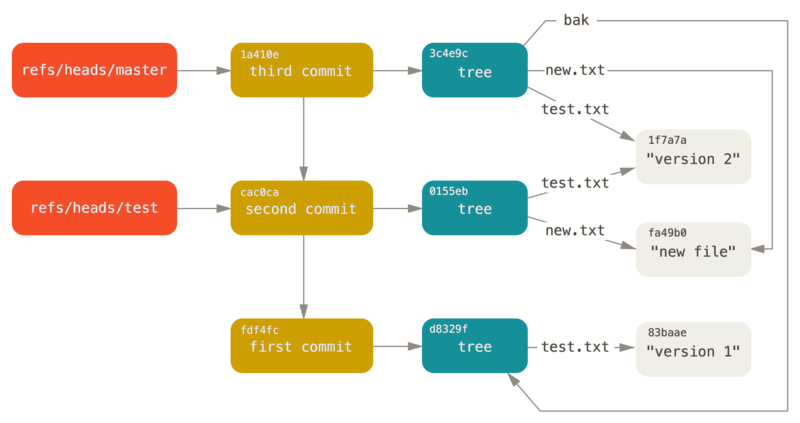
\includegraphics[width=\textwidth]{data-model-4.png}
    \label{fig:reference}
  \end{figure}
  When you run commands like \code{git branch <branch>},
  Git basically runs update-ref command to add the SHA-1
  of the last commit of the branch you're on into whatever
  new reference you want to create.
  So create branch is just create a reference to some commit.
  And delete branch is only delete reference.
  After branch deletion, all its objects will be available via their SHA.
  The same is for other reference under .git/refs
  \item[HEAD] Usually the HEAD file is a symbolic reference to the branch
  you're currently on.
  By symbolic reference, we mean that unlike a normal reference,
  it contains a pointer to another reference.\\
  If you look at the file, you'll normally see something like this:\\
  \\
  \code{\$ cat .git/HEAD}\\
  \code{ref: refs/heads/master}\\
  \\If you run \code{git checkout branch}, Git updates the file to look like this:\\
  \\
  \code{\$ cat .git/HEAD}\\
  \code{ref: refs/heads/test}\\

  When you run \code{git commit}, it creates the commit object,
  specifying the parent of that commit object to be whatever SHA-1 value
  the reference in HEAD points to.
  This commit also becomes a new head for a current branch.
  refs/heads/<branch-name> will be updated and map to the SHA
  of this new commit.
  When you do \code{git reset HEAD~1},
  it also only update refs/heads/<branch-name>.
  It takes SHA of parent commit of current head commit.
  \item[Tag (lightweight)] It's like a branch reference, but it never moves - it always points to the same commit but gives it a friendlier name.\\
  You can create, update and delete such a tag, and no objects would be affected.
  It's only a reference.
  \item[Tag (annotated)] - tag object, that points to commit or any other object amd contains metadata, and a reference to this tag object.

  Use \code{git push --follow-tags} if you want to push your annotated tag to remote repo.
  To delete a tag on your local repository, you can use \code{git tag -d <tagname>}.
  To delete a remote tag: \code{git push origin --delete <tagname>}.

  Both operation only delete a reference in .git/refs/tag.
  Tag object wouldn't be removed.
\end{description}

\subsubsection{Objects update workflow}
The most important updates of remote repo for us listed in the table below:

\begin{table}[H]
  \hskip-2.0cm\begin{tabular}{|l|l|l|}
                \hline
                action                                                               & git commands                                                                                                                                                                                                                                    & git server changes                                                                                                                                                                                                                                        \\ \hline
                create branch                                                        & \begin{tabular}[c]{@{}l@{}}git push  \textless{}remote-name\textgreater \\  \textless{}branch-name\textgreater{}:\textless{}remote-branch-name\textgreater{}\end{tabular}                                                                       & \begin{tabular}[c]{@{}l@{}}A new reference \\ .git/refs/heads/\textless{}branch-name\textgreater \\ will be created.\end{tabular}                                                                                                                         \\ \hline
                delete branch                                                        & \begin{tabular}[c]{@{}l@{}}git push  \textless{}remote-name\textgreater \\ :\textless{}remote-branch-name\textgreater\\ OR\\ git push \textless{}remote-name\textgreater  \\ --delete  \textless{}remote-branch-name\textgreater{}\end{tabular} & \begin{tabular}[c]{@{}l@{}}The existing reference \\ .git/refs/heads/\textless{}branch-name\textgreater \\ will be removed.\end{tabular}                                                                                                                  \\ \hline
                create tag                                                           & \begin{tabular}[c]{@{}l@{}}git push \textless{}remote-name\textgreater \\ \textless{}tag-name\textgreater{}:\textless{}remote-tag-name\textgreater{}\end{tabular}                                                                               & \begin{tabular}[c]{@{}l@{}}A new reference \\ .git/refs/tags/\textless{}tag-name\textgreater \\ will be created.\\ For annotated tags only:\\ new tag-object also will be created\\ .git/objects/SHA{[}0,2{]}/SHA{[}2,40{]}\end{tabular}                  \\ \hline
                delete tag                                                           & git push \textless{}remote-name\textgreater :\textless{}tag-name\textgreater{}                                                                                                                                                                  & \begin{tabular}[c]{@{}l@{}}The existing reference \\ .git/refs/tags/\textless{}tag-name\textgreater\\  will be removed.\\ For annotated tags:\\ tag-object won't be removed or updated\\ For lightweight tags:\\ tag-object doesn't exist\end{tabular}    \\ \hline
                \begin{tabular}[c]{@{}l@{}}create ref\\ delete ref\end{tabular}      &                                                                                                                                                                                                                                                 & \begin{tabular}[c]{@{}l@{}}Reference is fully equal to branch,\\  it's just an alias.\end{tabular}                                                                                                                                                        \\ \hline
                \begin{tabular}[c]{@{}l@{}}update branch\\ (new commit)\end{tabular} & git push                                                                                                                                                                                                                                        & \begin{tabular}[c]{@{}l@{}}New objects will be created \\ (commit, tree, etc.).\\ The existing reference \\ .git/refs/heads/\textless{}remote-branch-name\textgreater \\ will be updated.\\ It will start pointing \\ to to this new commit.\end{tabular} \\ \hline
  \end{tabular}\label{tab:update-workflow}
\end{table}

\section{Requirements}
\label{sec:requirements}

\subsection{Features}
\label{sec:features}

The most critical
\href{https://en.wikipedia.org/wiki/Non-functional_requirement}{Non-functional requirements}
are:

\begin{description}
  \item[Read scalability]
    The solution should scale out the read capacity of a system, each region should be able
    to access repository using most available replica node.
  \item[Strong consistency]
    All? (\todo{discuss, maybe not all but the majority of replicas})
    active replica repositories should be synchronized on updates in any node
    with immediate consistency.
  \item[Durability]
    The system must have enough replicas to recover itself in case of corruption.
    Corrupted repository could be responsible for recovering itself using replica nodes.
  \item[Self management (rename?)]
    Each node performs cleanup when needed (\code{git gc}) and may remove replica
    from storage on read inactivity.
    A node should be able to find and synchronize new repository on read,
    after that it should be up to date on new updates.
  \item[Maintainability]
    Node administrator can change the storage, and perform data migration from one storage
    to another.
    Repository administrators are able to add or delete node for new region and
    get all nodes status for repository.
  \item[Auditability]
    Node doesn't perform access control operations, but logs all
    requests with identity and performed operation.
  \item[Analytics]
    Node collects statistics for each repository and usage metrics, such as
    push and pull operations, etc. The system keeps the whole statistics about
    nodes, e.g. how many nodes contains each repository, the state of nodes, etc.
\end{description}


\section{Compare to other solutions}

These products are similar to DeGit by some aspects:
\begin{description}
  \item[Spokes]
    GitHub announced \href{https://github.blog/2016-04-05-introducing-dgit/}{DGit}
    in 2016 (renamed to \href{https://github.blog/2016-09-07-building-resilience-in-spokes/}{Spokes})
    where they \href{https://github.blog/2016-09-07-building-resilience-in-spokes/#defining-resilience}{pay attention}
    to the consistency:
    \begin{quote}
      Spokes puts the highest priority on consistency and partition tolerance.
      In worst-case failure scenarios, it will refuse to accept writes that it cannot commit,
      synchronously, to at least two replicas.
    \end{quote}
    It's a proprietary software that can't be used for free and the source code is closed.
    Spokes papers claims that it pays attention to consistency, but on the
    \href{https://www.youtube.com/watch?v=DY0yNRNkYb0}{conference talk} they mentioned that
    it's rarely possible to break the consistency which requires manual intervention.
    Therefore the approach of distributed system design used by Spokes is not suitable for open
    source project, where maintainance team doesn't exist.
  \item[Gitaly]
    \href{https://docs.gitlab.com/ee/README.html}{Gitlab} has
    \href{https://docs.gitlab.com/ee/administration/gitaly/}{Gitaly} service which provides
    \code{gRPC} API for Gitlab website and git-ssh proxy to perform all git operations via API.
    It's \href{https://gitlab.com/gitlab-org/gitaly}{open source} component.
    Gitaly proposed new design for service which claims to provide
    \href{https://gitlab.com/gitlab-org/gitaly/-/blob/master/doc/design\_ha.md\#strong-consistency-design}{strong concistency}
    but in fact it doesn't provide linearability of commands in system \todo{arguments and proves}.
    Futhermore, it's possible that GitLab may change HA licensing \todo{find cases},
    or restrict HA support \href{https://news.ycombinator.com/item?id=21437334}{based on country residence}.
  \item[JGit]
    \href{https://www.eclipse.org/jgit/}{Jgit} is a Java git server created by \href{https://www.eclipse.org/}{Eclipse}.
    Google \href{https://www.eclipse.org//lists/jgit-dev/msg03073.html}{contributed} to this project with Ketch module:
    \begin{quote}
      Git Ketch is a multi-master Git repository management system. Writes
      (such as git push) can be started on any server, at any time. Writes
      are successful only if a majority of participant servers agree.
      Acked writes are durable against server failure, due to a majority of
      the participants storing all required objects.
    \end{quote}
    But this is the only place where Ketch is mentioned. \todo{Analyze source code of Ketch module}.
  \item[IPFS]
    \href{https://ipfs.io/}{IPFS} is not exactly distributed git repository project, but has similar ideas
    and cound be helpfull for us. \todo{analyze IPFS project}.
  \item[brig]
    \todo{analyze the project} \href{https://github.com/sahib/brig}{brig}.
\end{description}

\subsection{Functional Requirements}
\label{sec:nfr}

The most important \href{https://en.wikipedia.org/wiki/Functional_requirement}{functional requirements} are:

\begin{description}
  \item[Front end]
    The system potentically may have different kinds of front-ends,
    but it's required to support \href{https://grpc.io/}{gRPC}
    of \href{https://about.gitlab.com/}{GitLab} to integrate the system
    into GitLab service and replace
    \href{https://docs.gitlab.com/ee/administration/gitaly/}{Gitaly}.
  \item[Back end]
    Each node may be connected to different types of storage for git repos,
    but it's required to support file-system storage.
\end{description}

\subsection{Expected Metrics}
\label{ref:metrics}

In a large enterprise it is expected to have the following
numbers, in terms of load, size, and speed:

\begin{tabular}{ll}
  Repositories & 2M \\
  Active users & 100K/day \\
  Merges & 100K/day \\
  Fetches & 15M/day, 15K/m - peak \\
  Push & 200K/day \\
  Traffic - download & 200Tb/day \\
  Traffic - update & 250Gb/day \\
\end{tabular}

\printbibliography%
\end{document}
